\documentclass[a4paper]{article}

\usepackage{Sweave} %--------------------------------!
\usepackage{amsmath}
\usepackage{amssymb}
\usepackage{amsthm}
\usepackage{fancyhdr}
\usepackage[usenames, dvipsnames]{color}
\usepackage{verbatim}

\oddsidemargin0cm
\topmargin-2cm     %I recommend adding these three lines to increase the
\textwidth16.5cm   %amount of usable space on the page (and save trees)
\textheight23.5cm

\newcommand{\question}[2] {\vspace{.25in} \hrule\vspace{0.5em}
\noindent{\bf #1: #2} \vspace{0.5em}
\hrule \vspace{.10in}}
\renewcommand{\part}[1] {\vspace{.10in} {\bf (#1)}}

\newcommand{\myname}{Xuan Han}
\newcommand{\myhusky}{han.xua@husky.neu}
\newcommand{\myhwnum}{2}

\setlength{\parindent}{0pt}
\setlength{\parskip}{5pt plus 1pt}

\pagestyle{fancyplain}
\lhead{\fancyplain{}{\textbf{HW\myhwnum}}}      % Note the different brackets!
\rhead{\fancyplain{}{\myname\\ \myhusky}}
\chead{\fancyplain{}{10 8 11}}


\begin{document}
\Sconcordance{concordance:lm.tex:lm.Rnw:%
1 47 1 1 2 1 0 1 1 32 0 1 1 19 0 1 1 3 0 1 2 10 1 1 2 1 0 6 1 4 0 1 2 %
13 1 1 2 5 0 1 2 4 1 1 2 1 0 3 1 4 0 1 3 1 0 4 1 6 0 1 1 6 0 1 1 8 0 1 %
2 11 1 1 2 7 0 1 2 4 1 1 2 8 0 1 2 4 1 1 2 11 0 1 1 9 0 1 2 9 1 1 2 6 0 %
1 1 5 0 2 1 8 0 1 1 10 0 1 2 12 1 1 2 1 0 3 1 21 0 2 1 6 0 1 1 7 0 1 1 %
6 0 1 1 7 0 1 2 9 1 1 2 1 0 1 1 4 0 1 2 3 1 1 2 1 0 1 1 4 0 1 2 7 1 1 2 %
1 0 2 1 3 0 1 2 1 1 1 2 1 0 1 1 20 0 2 1 4 0 1 2 14 1 1 2 1 0 1 1 20 0 %
2 1 4 0 1 2 38 1 1 2 7 0 1 2 5 1 1 2 1 0 1 1 21 0 1 2 1 1 22 0 1 2 6 1}


\title{Data Mining Assignment \myhwnum}
\author{\myname \\
        \myhusky}
\date{\today}
\maketitle

\medskip
\thispagestyle{plain}

\question{10}{Boston data set explore}
\part{a}
First, have a look at the dataset.
\begin{Schunk}
\begin{Sinput}
> library(MASS)
> summary(Boston)
\end{Sinput}
\begin{Soutput}
      crim                zn             indus            chas        
 Min.   : 0.00632   Min.   :  0.00   Min.   : 0.46   Min.   :0.00000  
 1st Qu.: 0.08204   1st Qu.:  0.00   1st Qu.: 5.19   1st Qu.:0.00000  
 Median : 0.25651   Median :  0.00   Median : 9.69   Median :0.00000  
 Mean   : 3.61352   Mean   : 11.36   Mean   :11.14   Mean   :0.06917  
 3rd Qu.: 3.67708   3rd Qu.: 12.50   3rd Qu.:18.10   3rd Qu.:0.00000  
 Max.   :88.97620   Max.   :100.00   Max.   :27.74   Max.   :1.00000  
      nox               rm             age              dis        
 Min.   :0.3850   Min.   :3.561   Min.   :  2.90   Min.   : 1.130  
 1st Qu.:0.4490   1st Qu.:5.886   1st Qu.: 45.02   1st Qu.: 2.100  
 Median :0.5380   Median :6.208   Median : 77.50   Median : 3.207  
 Mean   :0.5547   Mean   :6.285   Mean   : 68.57   Mean   : 3.795  
 3rd Qu.:0.6240   3rd Qu.:6.623   3rd Qu.: 94.08   3rd Qu.: 5.188  
 Max.   :0.8710   Max.   :8.780   Max.   :100.00   Max.   :12.127  
      rad              tax           ptratio          black       
 Min.   : 1.000   Min.   :187.0   Min.   :12.60   Min.   :  0.32  
 1st Qu.: 4.000   1st Qu.:279.0   1st Qu.:17.40   1st Qu.:375.38  
 Median : 5.000   Median :330.0   Median :19.05   Median :391.44  
 Mean   : 9.549   Mean   :408.2   Mean   :18.46   Mean   :356.67  
 3rd Qu.:24.000   3rd Qu.:666.0   3rd Qu.:20.20   3rd Qu.:396.23  
 Max.   :24.000   Max.   :711.0   Max.   :22.00   Max.   :396.90  
     lstat            medv      
 Min.   : 1.73   Min.   : 5.00  
 1st Qu.: 6.95   1st Qu.:17.02  
 Median :11.36   Median :21.20  
 Mean   :12.65   Mean   :22.53  
 3rd Qu.:16.95   3rd Qu.:25.00  
 Max.   :37.97   Max.   :50.00  
\end{Soutput}
\begin{Sinput}
> str(Boston)
\end{Sinput}
\begin{Soutput}
'data.frame':	506 obs. of  14 variables:
 $ crim   : num  0.00632 0.02731 0.02729 0.03237 0.06905 ...
 $ zn     : num  18 0 0 0 0 0 12.5 12.5 12.5 12.5 ...
 $ indus  : num  2.31 7.07 7.07 2.18 2.18 2.18 7.87 7.87 7.87 7.87 ...
 $ chas   : int  0 0 0 0 0 0 0 0 0 0 ...
 $ nox    : num  0.538 0.469 0.469 0.458 0.458 0.458 0.524 0.524 0.524 0.524 ...
 $ rm     : num  6.58 6.42 7.18 7 7.15 ...
 $ age    : num  65.2 78.9 61.1 45.8 54.2 58.7 66.6 96.1 100 85.9 ...
 $ dis    : num  4.09 4.97 4.97 6.06 6.06 ...
 $ rad    : int  1 2 2 3 3 3 5 5 5 5 ...
 $ tax    : num  296 242 242 222 222 222 311 311 311 311 ...
 $ ptratio: num  15.3 17.8 17.8 18.7 18.7 18.7 15.2 15.2 15.2 15.2 ...
 $ black  : num  397 397 393 395 397 ...
 $ lstat  : num  4.98 9.14 4.03 2.94 5.33 ...
 $ medv   : num  24 21.6 34.7 33.4 36.2 28.7 22.9 27.1 16.5 18.9 ...
\end{Soutput}
\begin{Sinput}
> attach(Boston)
\end{Sinput}
\end{Schunk}

\begin{enumerate}
{
\color{red}
\item The Boston data frame has 506 rows and 14 columns.
\item All of the colnums are numerical values, which contains quantitive information like crime rate, nitrogen oxides concentration, average room number, age, tax.
\item However, there is one colnum feature, chas, is actually a binary YES/NO category value which is represented by 1/0.
}
\end{enumerate}

\part{b}
\begin{Schunk}
\begin{Sinput}
> par(mfrow = c(3,2))
> boxplot(crim ~ chas, main = "chas vs. crime", col = rainbow(7), xlab = "chas", ylab = "crime")
> plot(y = medv, x = rm, main = "medv vs. rm", col = rainbow(7), ylab = "medv", xlab = "rm")
> plot(y = nox, x = dis, main = "nox vs. dis", col = rainbow(7), ylab = "nox", xlab = "dis")
> plot(y = nox, x = age, main = "nox vs. age", col = rainbow(7), ylab = "nox", xlab = "age")
> plot(y = crim, x = rad, main = "crim vs. rad", col = rainbow(7), ylab = "crim", xlab = "rad")
> plot(y = rm, x = tax, main = "rm vs. tax", col = rainbow(7), ylab = "rm", xlab = "tax")
\end{Sinput}
\end{Schunk}
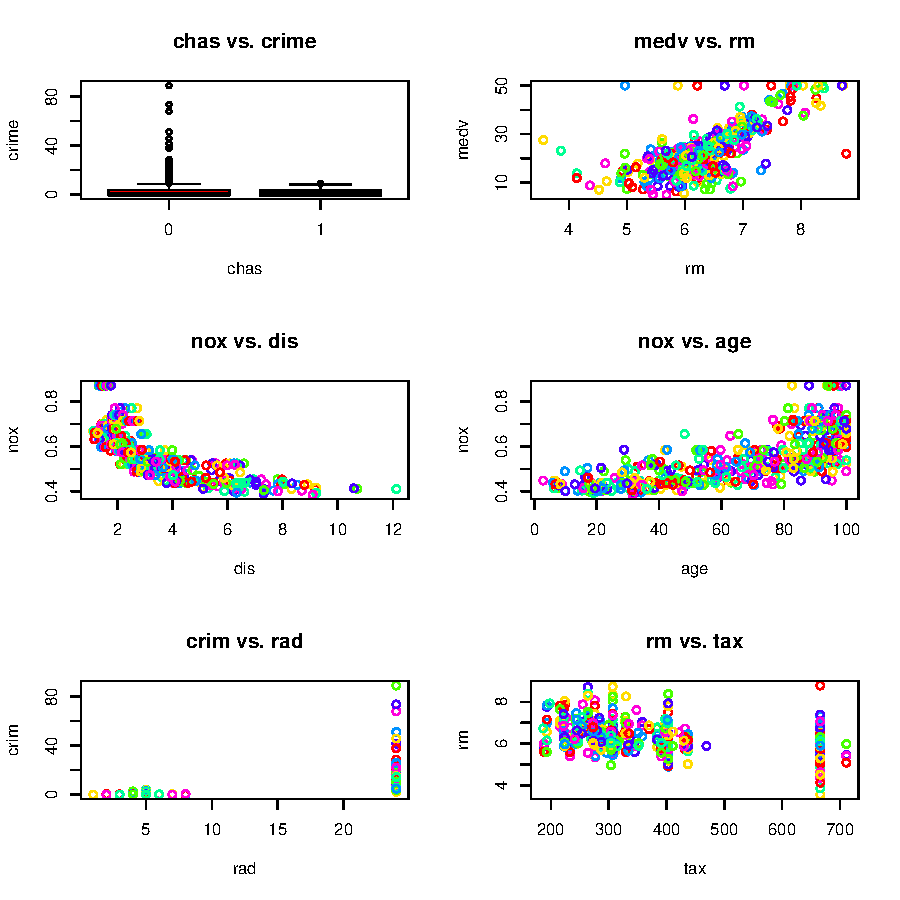
\includegraphics{lm-pairboston}
\begin{enumerate}
{
\color{red}
\item we can see the crime rate in Boston is low in overall. However, places not bounded with Charles River are more likely have higher crime rate.
\item The more room number, the higher the median value of the house.
\item The futher the distance from downtown, the lower nitrogen oxides concentration
\item The more propotion of old house, the higher nitrogen oxides concentration
\item It seems within 10 unit accessibility to radial highways the crime is low, it goes ridicaly when the index pass 20.
\item It seems there is no obvious relationship between tax and room number.
}
\end{enumerate}

\part{c}
Yes, there are. Just as I have described in (b), Charles River and rad are good predictors. Besides, I find that distance to Boston employment centres is also a good predictor.
\begin{Schunk}
\begin{Sinput}
> plot(y = crim, x = dis, main = "crim vs. dis", col = rainbow(7), ylab = "crim", xlab = "dis")
\end{Sinput}
\end{Schunk}
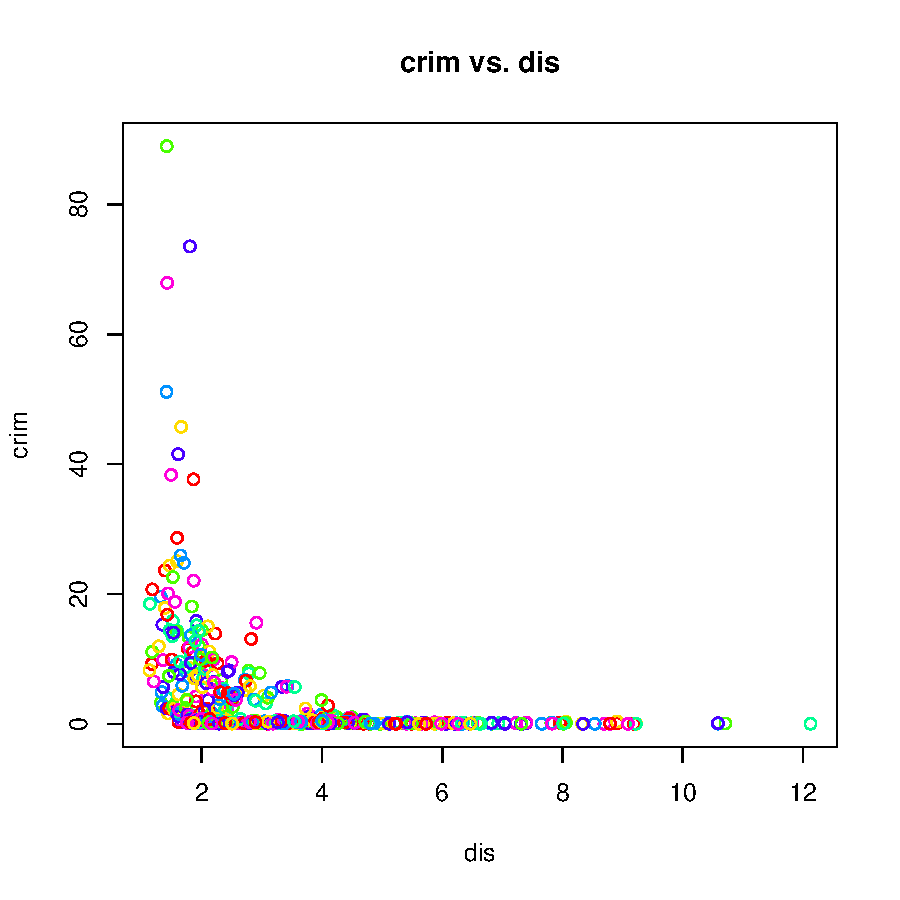
\includegraphics{lm-crime}
{\color{red}\\
I find that when the distance is around 2 unit, the crime rate is very hight. With distance goes on, crime rate keep at the same level.
}

\part{d}
\begin{Schunk}
\begin{Sinput}
> par(mfrow = c(1, 3))
> boxplot(crim, col = rainbow(7), main = "crime rate")
> boxplot(tax, col = rainbow(7), main = "tax rate")
> boxplot(ptratio, col = rainbow(7), main = "pupil-teacher ratio")
\end{Sinput}
\end{Schunk}
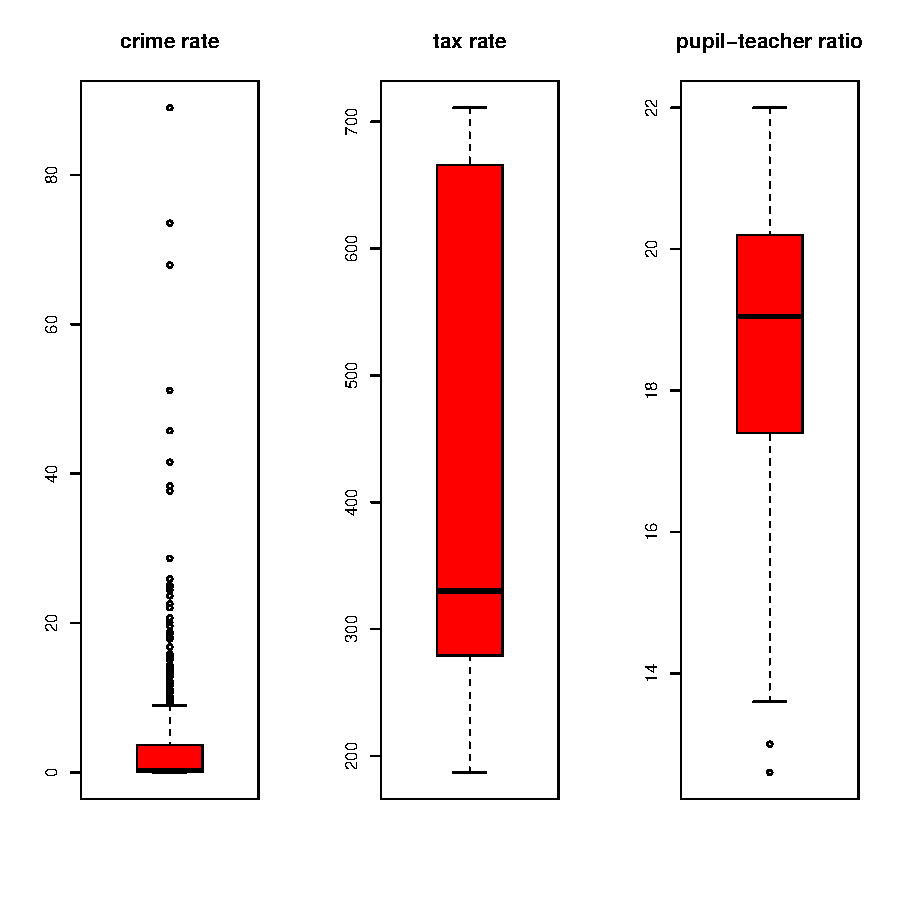
\includegraphics{lm-high}
\begin{Schunk}
\begin{Sinput}
> par(mfrow = c(1, 3))
> hist(crim)
> hist(tax)
> hist(ptratio)
> summary(crim)
\end{Sinput}
\begin{Soutput}
    Min.  1st Qu.   Median     Mean  3rd Qu.     Max. 
 0.00632  0.08204  0.25650  3.61400  3.67700 88.98000 
\end{Soutput}
\begin{Sinput}
> summary(tax)
\end{Sinput}
\begin{Soutput}
   Min. 1st Qu.  Median    Mean 3rd Qu.    Max. 
  187.0   279.0   330.0   408.2   666.0   711.0 
\end{Soutput}
\begin{Sinput}
> summary(ptratio)
\end{Sinput}
\begin{Soutput}
   Min. 1st Qu.  Median    Mean 3rd Qu.    Max. 
  12.60   17.40   19.05   18.46   20.20   22.00 
\end{Soutput}
\end{Schunk}
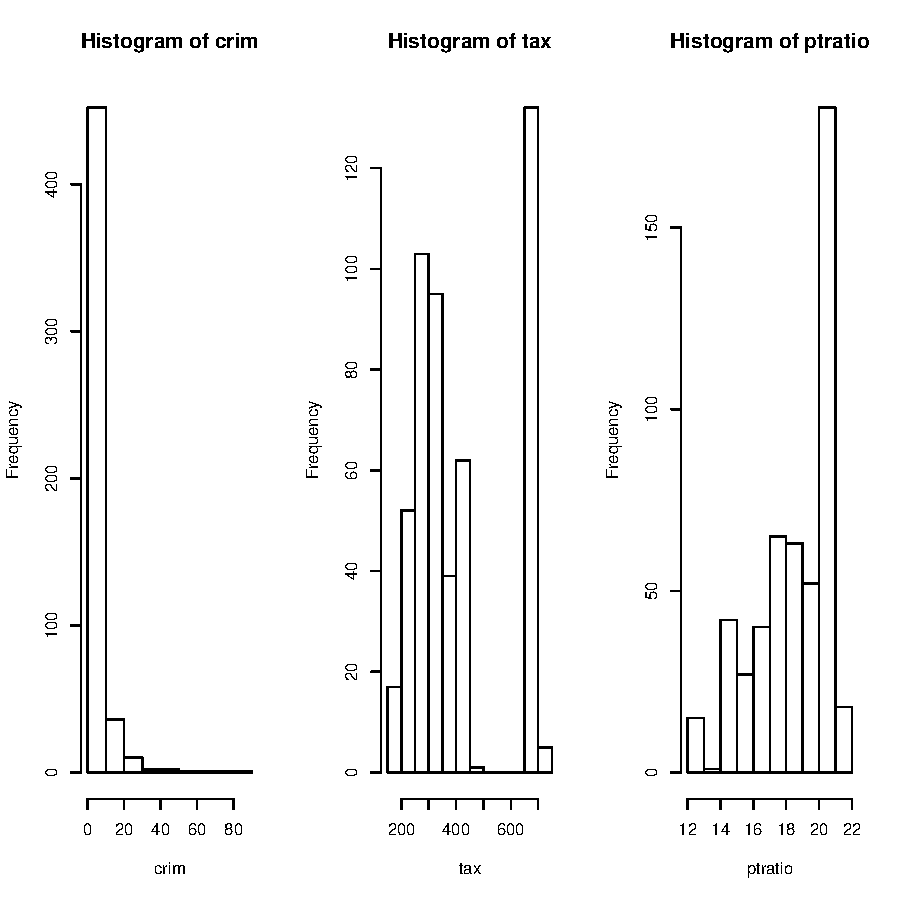
\includegraphics{lm-hist}
\begin{enumerate}
{\color{red}
\item We can see that some subursbs of Boston really have particularly high crime rate and tax rate. But not pupil-teacher ratios. Instead, there are particularly low pupil-teacher ratios.
\item For both crime rate and tax rate, there are instances that are far away from there median value.
\item The range of crime is between 0.00632 and 88.9, the gap is quite huge. This means there are very good areas and extremly bad areas. Fortunately, for most of the areas the crime rate is below 10.
\item The range of tax is between 187 and 711. But we dont have data about tax between 500 to 600. There are also very high tax rate that away from the median of the data set.
\item The range of pupil-teacher ratio is between 12.6 and 22, which is not a huge gap. This means the resources of education is relatively fare.
}
\end{enumerate}


\part{e}
\begin{Schunk}
\begin{Sinput}
> sum(Boston$chas)
\end{Sinput}
\begin{Soutput}
[1] 35
\end{Soutput}
\end{Schunk}
{\color{red}
35 suburbs are bounded to Charles River.}


\part{f}
\begin{Schunk}
\begin{Sinput}
> summary(ptratio)
\end{Sinput}
\begin{Soutput}
   Min. 1st Qu.  Median    Mean 3rd Qu.    Max. 
  12.60   17.40   19.05   18.46   20.20   22.00 
\end{Soutput}
\end{Schunk}
{\color{red}
The median pupil-teacher ratio among the towns in this data set is 19.05}


\part{g}
\begin{Schunk}
\begin{Sinput}
> Boston[Boston$medv == summary(medv)[1],]
\end{Sinput}
\begin{Soutput}
       crim zn indus chas   nox    rm age    dis rad tax ptratio  black lstat
399 38.3518  0  18.1    0 0.693 5.453 100 1.4896  24 666    20.2 396.90 30.59
406 67.9208  0  18.1    0 0.693 5.683 100 1.4254  24 666    20.2 384.97 22.98
    medv
399    5
406    5
\end{Soutput}
\begin{Sinput}
> round(sapply(Boston, mean), 2)
\end{Sinput}
\begin{Soutput}
   crim      zn   indus    chas     nox      rm     age     dis     rad     tax 
   3.61   11.36   11.14    0.07    0.55    6.28   68.57    3.80    9.55  408.24 
ptratio   black   lstat    medv 
  18.46  356.67   12.65   22.53 
\end{Soutput}
\end{Schunk}

\begin{enumerate}
{\color{red}
\item subsurb 399 and 406 have the lowest medv, which is 5
\item Compared with other areas, these two areas have very high crim rate, much higher zn index, with more non-retail business. Those houses in the two areas are very old. They are far away from radial highways, with lower lstat.
}
\end{enumerate}


\part{h}
\begin{Schunk}
\begin{Sinput}
> sum(Boston$rm > 7)
\end{Sinput}
\begin{Soutput}
[1] 64
\end{Soutput}
\begin{Sinput}
> sum(Boston$rm > 8)
\end{Sinput}
\begin{Soutput}
[1] 13
\end{Soutput}
\begin{Sinput}
> boxplot(Boston[Boston$rm > 8,])
> round(sapply(Boston[Boston$rm > 8,], mean), 2)
\end{Sinput}
\begin{Soutput}
   crim      zn   indus    chas     nox      rm     age     dis     rad     tax 
   0.72   13.62    7.08    0.15    0.54    8.35   71.54    3.43    7.46  325.08 
ptratio   black   lstat    medv 
  16.36  385.21    4.31   44.20 
\end{Soutput}
\begin{Sinput}
> round(sapply(Boston, mean), 2)
\end{Sinput}
\begin{Soutput}
   crim      zn   indus    chas     nox      rm     age     dis     rad     tax 
   3.61   11.36   11.14    0.07    0.55    6.28   68.57    3.80    9.55  408.24 
ptratio   black   lstat    medv 
  18.46  356.67   12.65   22.53 
\end{Soutput}
\end{Schunk}
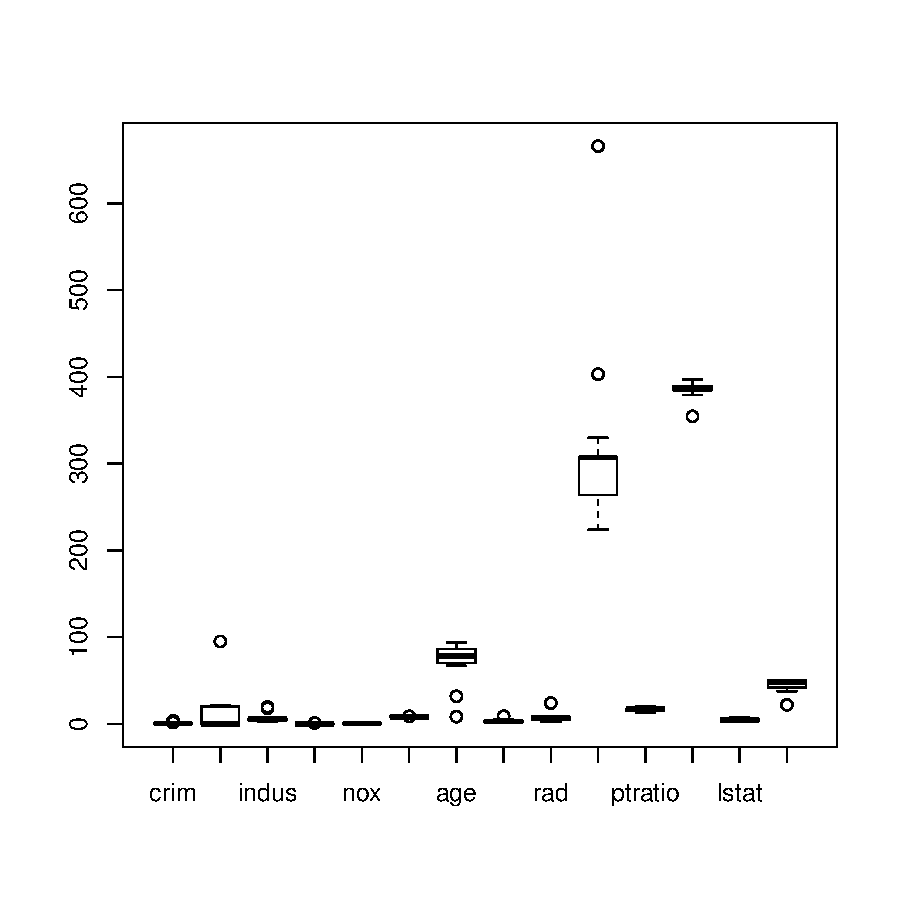
\includegraphics{lm-dewlling}

\begin{enumerate}
{\color{red}
\item 64 suburbs average more than seven rooms per dwelling
\item 13 suburbs average more than eight rooms per dwelling
\item Compared with other areas, these areas have much less crime rate, lower lstat index, but much higher medv. These areas have less people and much safer.
}
\end{enumerate}



\question{8}{lm on Auto}
\part{a}
\begin{Schunk}
\begin{Sinput}
> library(ISLR)
> attach(Auto)
> fit = lm(mpg ~ horsepower, data = Auto)
> summary(fit)
\end{Sinput}
\begin{Soutput}
Call:
lm(formula = mpg ~ horsepower, data = Auto)

Residuals:
     Min       1Q   Median       3Q      Max 
-13.5710  -3.2592  -0.3435   2.7630  16.9240 

Coefficients:
             Estimate Std. Error t value Pr(>|t|)    
(Intercept) 39.935861   0.717499   55.66   <2e-16 ***
horsepower  -0.157845   0.006446  -24.49   <2e-16 ***
---
Signif. codes:  0 ‘***’ 0.001 ‘**’ 0.01 ‘*’ 0.05 ‘.’ 0.1 ‘ ’ 1

Residual standard error: 4.906 on 390 degrees of freedom
Multiple R-squared:  0.6059,	Adjusted R-squared:  0.6049 
F-statistic: 599.7 on 1 and 390 DF,  p-value: < 2.2e-16
\end{Soutput}
\begin{Sinput}
> new.data = data.frame(horsepower = 98, mpg = 0)
> predict.lm(fit, new.data)
\end{Sinput}
\begin{Soutput}
       1 
24.46708 
\end{Soutput}
\begin{Sinput}
> confint(fit, level = 0.9)
\end{Sinput}
\begin{Soutput}
                   5 %       95 %
(Intercept) 38.7528707 41.1188513
horsepower  -0.1684719 -0.1472176
\end{Soutput}
\begin{Sinput}
> predict.lm(fit, new.data, interval = c('pred'))
\end{Sinput}
\begin{Soutput}
       fit     lwr      upr
1 24.46708 14.8094 34.12476
\end{Soutput}
\begin{Sinput}
> predict.lm(fit, new.data, interval = c('con'))
\end{Sinput}
\begin{Soutput}
       fit      lwr      upr
1 24.46708 23.97308 24.96108
\end{Soutput}
\end{Schunk}
\begin{enumerate}
{\color{red}
\item There for sure is a negative relationship between the reponse and predictor. The more horsepower, the less mpg.
\item At the begining, mpg decrease very quickly with horsepower increase. In the end, mpg does not change even horsepower increase.
\item pedicted value is 24.467, 95\% confidence interval is [23.97, 24.96] while predict interval is [14.81, 34,12]
}
\end{enumerate}


\part{b}
\begin{Schunk}
\begin{Sinput}
> plot(mpg ~ horsepower, data = Auto, col = "blue")
> abline(fit)
\end{Sinput}
\end{Schunk}
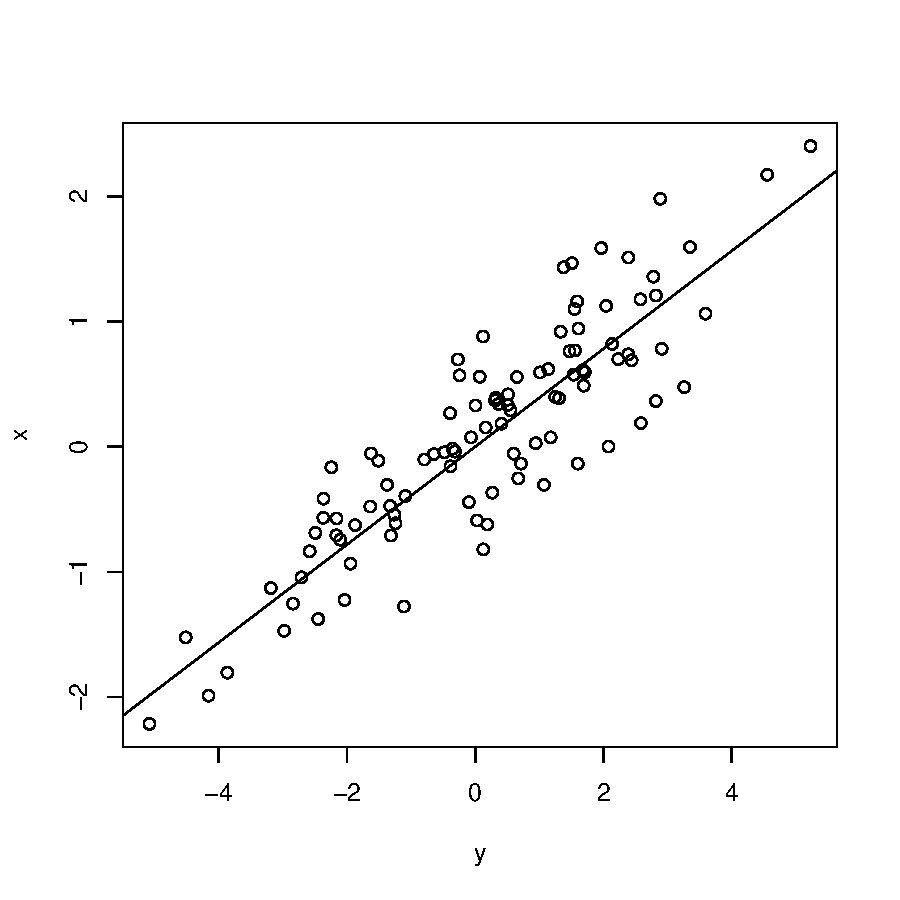
\includegraphics{lm-b}
{\color{red}\\ See above figure.}


\part{c}
\begin{Schunk}
\begin{Sinput}
> plot(residuals(fit))
> abline(h = 0)
\end{Sinput}
\end{Schunk}
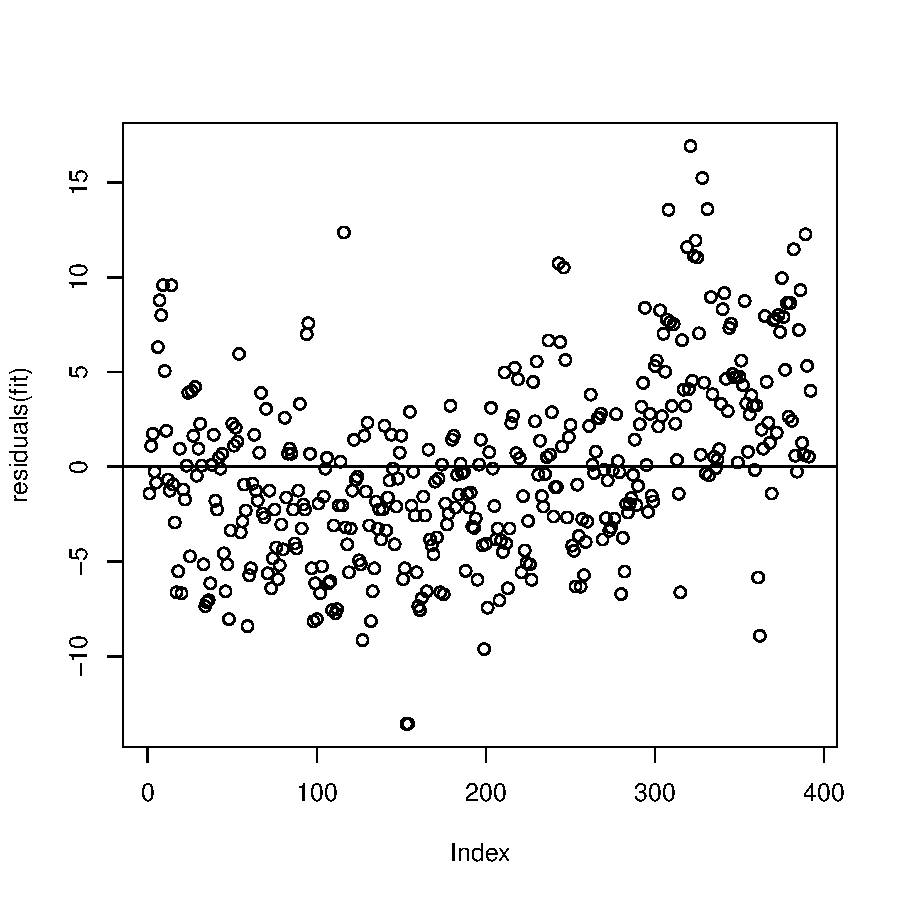
\includegraphics{lm-c}

{
\color{red}
From the residual plot we can see that the linear is not a good fit. The mean of the residual is not zero. For the left part, most of the resudial points are below the line while for the right part they are above the line.
}


\question{11}{t-statistic}
\begin{Schunk}
\begin{Sinput}
> set.seed(1)
> x = rnorm(100)
> y = 2 * x + rnorm(100)
\end{Sinput}
\end{Schunk}

\part{a}
\begin{Schunk}
\begin{Sinput}
> fit = lm(y ~ x + 0)
> summary(fit)
\end{Sinput}
\begin{Soutput}
Call:
lm(formula = y ~ x + 0)

Residuals:
    Min      1Q  Median      3Q     Max 
-1.9154 -0.6472 -0.1771  0.5056  2.3109 

Coefficients:
  Estimate Std. Error t value Pr(>|t|)    
x   1.9939     0.1065   18.73   <2e-16 ***
---
Signif. codes:  0 ‘***’ 0.001 ‘**’ 0.01 ‘*’ 0.05 ‘.’ 0.1 ‘ ’ 1

Residual standard error: 0.9586 on 99 degrees of freedom
Multiple R-squared:  0.7798,	Adjusted R-squared:  0.7776 
F-statistic: 350.7 on 1 and 99 DF,  p-value: < 2.2e-16
\end{Soutput}
\begin{Sinput}
> plot(x, y)
> abline(fit)
\end{Sinput}
\end{Schunk}
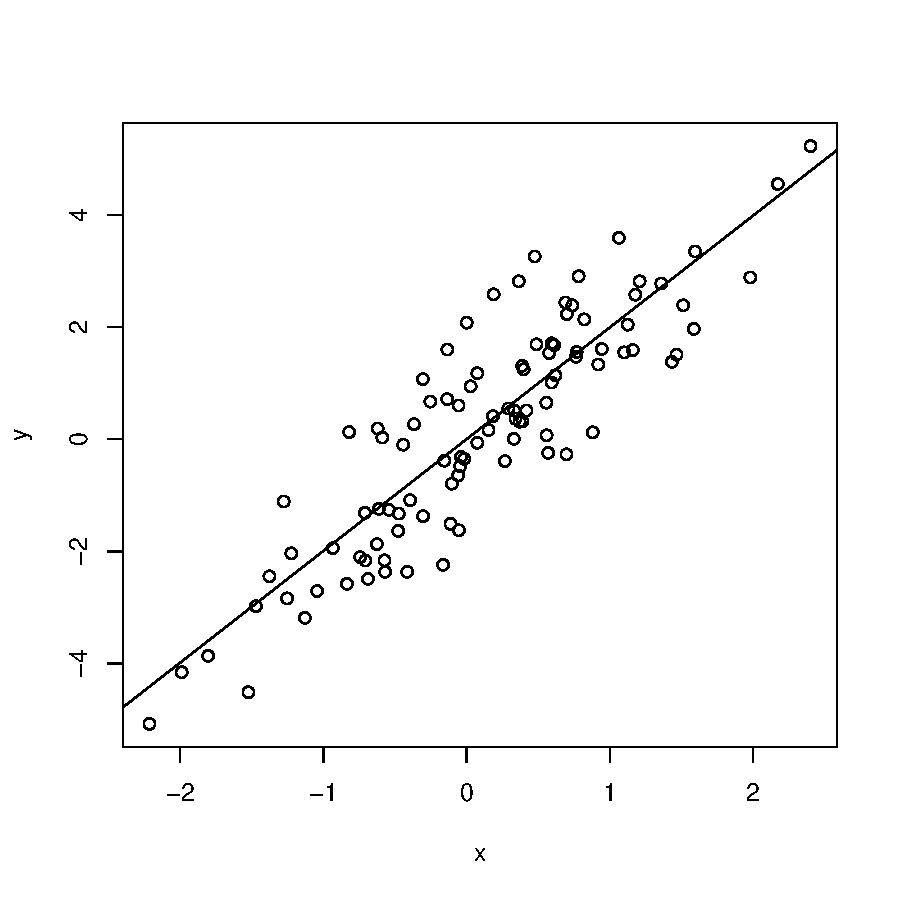
\includegraphics{lm-a}
\begin{enumerate}
{\color{red}
\item From the summary of the model, we can see that:
\begin{itemize}
\item estimated $\hat{\beta}$ is 1.9939
\item standard error of this coefficient estimate is 0.1065, small relatatively to $\hat{\beta}$
\item t-statistic is 18.73
\item p-value is $2.2 * 10^{-16}$
\end{itemize}
This result suppose that the null hypothesis: $H_0$ : $\beta = 0$ is rejected. There must be an association between x and y.
}
\end{enumerate}


\part{b}
\begin{Schunk}
\begin{Sinput}
> fit = lm(x ~ y + 0)
> summary(fit)
\end{Sinput}
\begin{Soutput}
Call:
lm(formula = x ~ y + 0)

Residuals:
    Min      1Q  Median      3Q     Max 
-0.8699 -0.2368  0.1030  0.2858  0.8938 

Coefficients:
  Estimate Std. Error t value Pr(>|t|)    
y  0.39111    0.02089   18.73   <2e-16 ***
---
Signif. codes:  0 ‘***’ 0.001 ‘**’ 0.01 ‘*’ 0.05 ‘.’ 0.1 ‘ ’ 1

Residual standard error: 0.4246 on 99 degrees of freedom
Multiple R-squared:  0.7798,	Adjusted R-squared:  0.7776 
F-statistic: 350.7 on 1 and 99 DF,  p-value: < 2.2e-16
\end{Soutput}
\begin{Sinput}
> plot(y, x)
> abline(fit)
\end{Sinput}
\end{Schunk}
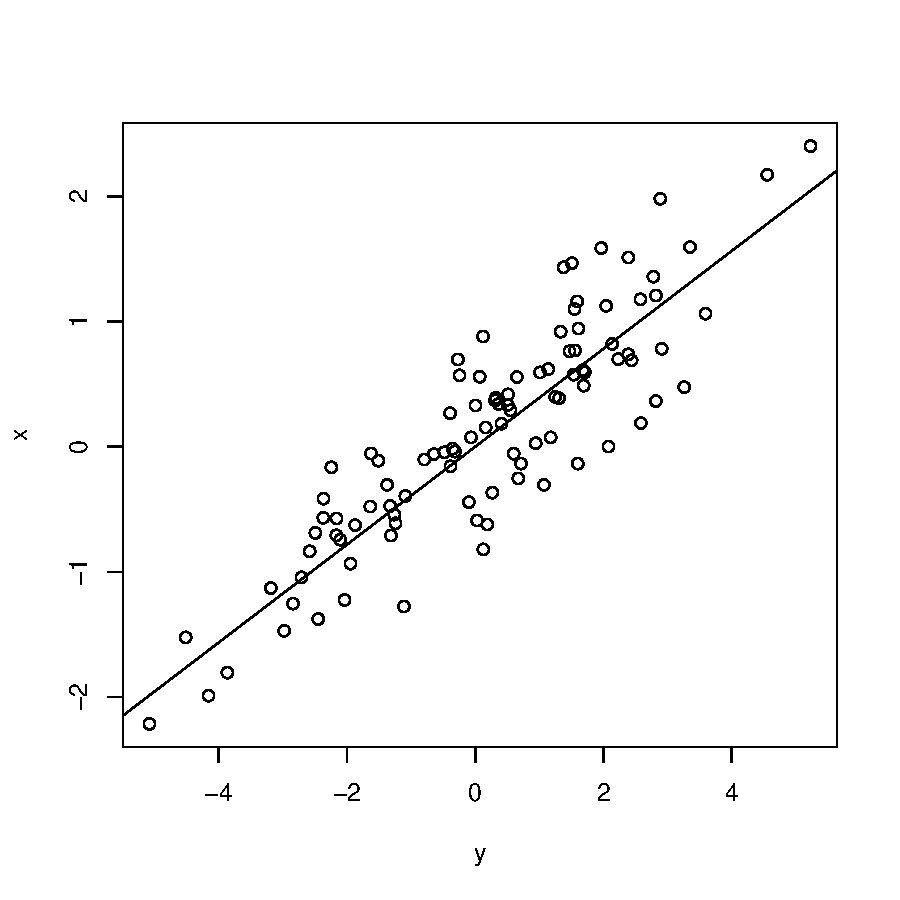
\includegraphics{lm-b}

\begin{enumerate}
{\color{red}
\item From the summary of the model, we can see that:
\begin{itemize}
\item estimated $\hat{\beta}$ is 0.39111
\item standard error of this coefficient estimate is 0.02089, small relatively to $\hat{\beta}$
\item t-statistic is 18.73
\item p-value is $2.2 * 10^{-16}$
\end{itemize}
Again, this result suppose that the null hypothesis: $H_0$ : $\beta = 0$ is rejected. There must be an association between x and y.
}
\end{enumerate}

\part{c}
\begin{enumerate}
{\color{red}
\item They have exactly the same t-value, r-squared, F-value and p-value.
\item They both rejected the null hypothesis
}
\end{enumerate}


\part{d}
\begin{proof}
Since x is generated with zero mean $\implies \bar{x} = \bar{y} = 0$\\
$\implies \beta = \frac{\sum_{i}^{n} x_iy_i}{\sum_{i}^{n}x_i^2}$\\
Thus:
\begin{eqnarray*}
t &=&\frac{\hat{\beta}}{SE(\hat{\beta})}\\
  &=&\frac{\sum_{i}^{n} x_iy_i}{\sum_{i}^{n}x_i^2} \sqrt{\frac{(n-1)\sum_i^n x_i^2}{\sum_i^n (y_i-x_i\hat{\beta})}}\\
  &=&\frac{\sqrt{n-1}\sum_i^n x_iy_i}{\sqrt{\sum_i^n x_i^2 \sum_i^n (y_i - x_i \hat{\beta})^2}}\\
  &=&\frac{\sqrt{n-1}\sum_i^n x_iy_i}{\sqrt{\sum_i^n x_i^2 \sum_i^n (y_i^2 + (x_i\hat{\beta})^2 - 2y_ix_i\hat{\beta})}}\\
  &=&\frac{\sqrt{n-1}\sum_i^n x_iy_i}{\sqrt{\sum_i^nx_i^2\sum_i^ny_i^2 - \sum_i^nx_i^2\hat{\beta}(2\sum_i^nx_iy_i - \hat{\beta}\sum_i^nx_i^2)}}\\
  &&now, plug in \hat{\beta}\\
  &=& \frac{\sqrt{n-1}\sum_i^n x_iy_i}{\sqrt{\sum_i^nx_i^2\sum_i^ny_i^2 - \sum_i^nx_iy_i(2\sum_i^nx_iy_i - \sum_i^nx_iy_i)}}\\
  &=& \frac{\sqrt{n-1}\sum_i^n x_iy_i}{\sqrt{\sum_i^nx_i^2\sum_i^ny_i^2 - (\sum_i^nx_iy_i)^2}}\\
\end{eqnarray*}
\end{proof}
\begin{Schunk}
\begin{Sinput}
> (sqrt(length(x) - 1) * sum(x*y)) / (sqrt(sum(x*x) * sum(y*y) - (sum(x*y)) ^ 2))
\end{Sinput}
\begin{Soutput}
[1] 18.72593
\end{Soutput}
\end{Schunk}

\part{e}
{\color{red}
This is pretty simple: the equation we inferred above is symmetric for both x and y. So change the postion of x and does not change t-value}

\part{f}
\begin{Schunk}
\begin{Sinput}
> fit = lm(y ~ x)
> summary(fit)
\end{Sinput}
\begin{Soutput}
Call:
lm(formula = y ~ x)

Residuals:
    Min      1Q  Median      3Q     Max 
-1.8768 -0.6138 -0.1395  0.5394  2.3462 

Coefficients:
            Estimate Std. Error t value Pr(>|t|)    
(Intercept) -0.03769    0.09699  -0.389    0.698    
x            1.99894    0.10773  18.556   <2e-16 ***
---
Signif. codes:  0 ‘***’ 0.001 ‘**’ 0.01 ‘*’ 0.05 ‘.’ 0.1 ‘ ’ 1

Residual standard error: 0.9628 on 98 degrees of freedom
Multiple R-squared:  0.7784,	Adjusted R-squared:  0.7762 
F-statistic: 344.3 on 1 and 98 DF,  p-value: < 2.2e-16
\end{Soutput}
\begin{Sinput}
> fit = lm(x ~ y)
> summary(fit)
\end{Sinput}
\begin{Soutput}
Call:
lm(formula = x ~ y)

Residuals:
     Min       1Q   Median       3Q      Max 
-0.90848 -0.28101  0.06274  0.24570  0.85736 

Coefficients:
            Estimate Std. Error t value Pr(>|t|)    
(Intercept)  0.03880    0.04266    0.91    0.365    
y            0.38942    0.02099   18.56   <2e-16 ***
---
Signif. codes:  0 ‘***’ 0.001 ‘**’ 0.01 ‘*’ 0.05 ‘.’ 0.1 ‘ ’ 1

Residual standard error: 0.4249 on 98 degrees of freedom
Multiple R-squared:  0.7784,	Adjusted R-squared:  0.7762 
F-statistic: 344.3 on 1 and 98 DF,  p-value: < 2.2e-16
\end{Soutput}
\end{Schunk}

{\color{red}
As shown above, the t-value for $\hat{\beta^1}$ are both 18.56
}

\end{document}
